%%%%%%%%%%
% PREAMBLE
%%%%%%%%%%

\documentclass{article}
\usepackage[utf8]{inputenc}
\usepackage[english]{babel}
\usepackage[style=numeric,sorting=ynt]{biblatex}
\usepackage[]{graphicx} % standard image package
\usepackage{svg} % include svg images
\usepackage{amsmath} % standard math package
\usepackage{float} % allow in place anchoring of images
\usepackage{multirow} % create nice tables
\usepackage{hyperref} % make links clickable

% Set up packages
\graphicspath{{../images/},{../images/movie_por0_stre6/},{../images/movie_por50_stre6/},{../images/movie_por50_stre3/},{../images/movie_por50_stre3_ang45/}}
\addbibresource{MasterThesis_References.bib}

% Commands
%\newcommand{\vec}{\boldsymbol}


%%%%%%%%%%
% INTRODUCTORY PAGES
%%%%%%%%%%
\begin{document}
\pagenumbering{roman}
\begin{titlepage}
    \begin{center}
        % \vspace*{.06\textheight}
        {\scshape\LARGE Eberhard Karls Universität Tübingen\par}\vspace{1.5cm} % University name
        \textsc{\Large Master Thesis}\\[0.5cm] % Thesis type
        \
        \hrule\ \\[0.0cm] % Horizontal line
        {\huge \bfseries Smoothed Particle Hydrodynamics Simulations for Asteroid Deflection\par}\vspace{0.8cm} % Thesis title
        \hrule\ \\[1.5cm] % Horizontal line
        \begin{minipage}[t]{0.4\textwidth}
            \begin{flushleft} \large
                \emph{Author:}\\
                {Maximilian Rutz}\\ % Author name - remove the \href bracket to remove the link
                Matrikelnr. 4255042
            \end{flushleft}
        \end{minipage}
        \begin{minipage}[t]{0.4\textwidth}
            \begin{flushright} \large
                \emph{Supervisor:}\\
                {Dr. Christoph Schäfer}\\
                {Prof. Dr. Wilhelm Kley} % Supervisor name - remove the \href bracket to remove the link
            \end{flushright}
        \end{minipage}\\[3cm]
        \vfill
        \large \textit{A thesis submitted in fulfillment of the requirements\\ for the Master of Science in Physics}\\[0.3cm] % University requirement text
        % \textit{in the}\\[0.4cm]
        \ \\[0.8cm]
        % Computational Physics - CPT\\
        Mathematisch-Naturwissenschaftliche Fakultät\\[2cm] % Research group name and department name
        \vfill
        {\large \today}\\[4cm] % Date
        %\includegraphics{Logo} % University/department logo - uncomment to place it
        \vfill
    \end{center}
\end{titlepage}
\thispagestyle{empty}
\newpage
\thispagestyle{plain}
\section*{Declaration}
I hereby declare that I have written the present thesis
independently, without assistance from external parties and without
use of other resources than those indicated.
The ideas taken directly or indirectly from external sources
(including electronic sources) are duly acknowledged in the text.
The material, either in full or in part, has not been previously
submitted for grading at this or any other academic institution.\\
\parbox{\textwidth}{
    \vspace{3cm}
    \parbox{7cm}{
        \rule{5cm}{0.5pt}\\
        Location, date
    }
    \hfill
    \parbox{7cm}{
        \rule{5cm}{0.5pt}\\
        Maximilian Rutz
    }
}
\newpage
\thispagestyle{plain}
\section*{ABSTRACT}
Fragen:


\thispagestyle{empty}
\newpage
\tableofcontents
\newpage
\pagenumbering{arabic}


%%%%%%%%%%
% BODY
%%%%%%%%%%

\newpage
\section{Introduction}
\begin{figure}[H]
    \centering
    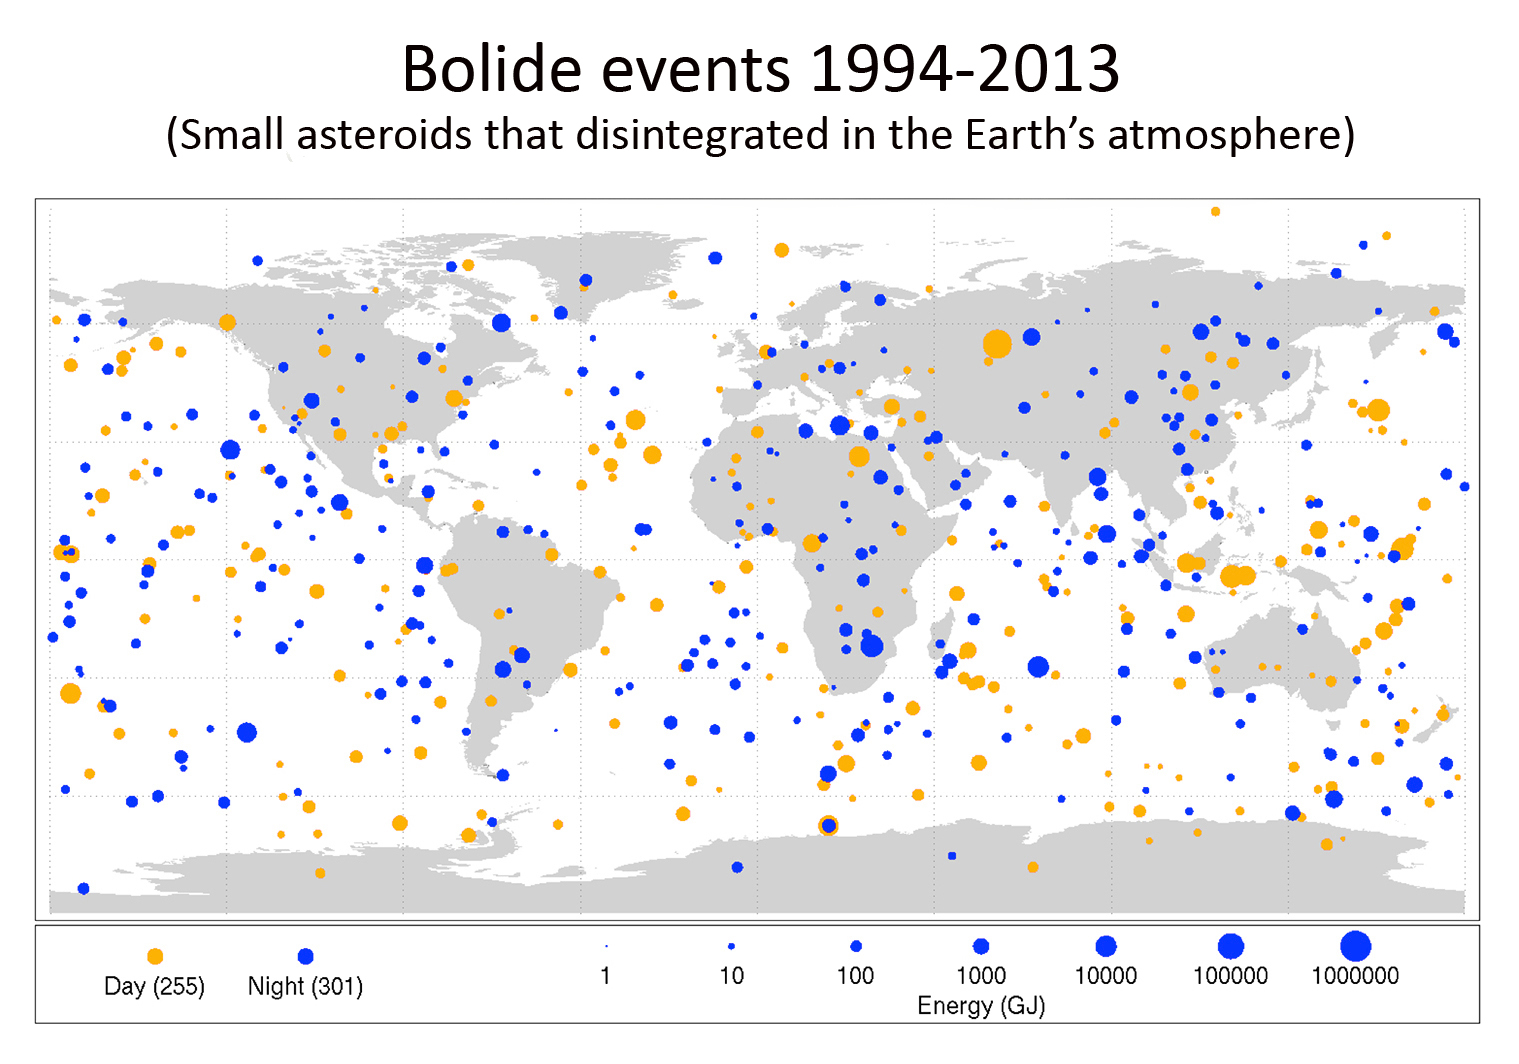
\includegraphics[width=\textwidth]{past_impacts.jpg}
    \caption{Past impacts \cite{wiki:past_impacts}}
    \label{fig:past_impacts}
\end{figure}


- test case for p-alpha porosity and pressure dependent yield strength

- Raducan \cite{Raducan_2019_strength} grid based 2d sims
- Stickle \cite{Stickle_2017}
\newpage
\section{Theory}
- Equations from Geophysics/Continuum Mechanics and High velocity impact physics that are needed to model the Impact

- all parameters that appear in the table of the Numerics section should be explained

\subsection{Conservation equations}
- mass
- momentum
- energy

\subsection{Constitutive equations}
- time evolution of deviatoric stress tensor


\subsection{Equation of State}
- Tillotson equation of state \cite{Tillotson_1962}

\subsection{Porosity model}
There are different ways in which porosity can be modeled depending on the pore size. Depending on the simulation, macro porosity with pore sizes above the resolution of the simulation can be accounted for in the initial conditions. This however becomes impossible for granular material with sub-resolution sized grains and pores.

Microporosity models porosity as an additional material property and can be applied independently of the resolution.


In these simulations, a microporosity p-$\alpha$ model as outlined in \cite{Jutzi_2008} is used. The distention $\alpha \in [1,\inf)$ relates the current density $\rho$ to the solid density $\rho_s$ which is reached if the material is fully compressed. For a non-porous material $\alpha$ equals one.

\begin{equation}
    \alpha \equiv \frac{\rho_s}{\rho}
\end{equation}

Often the porosity $\phi$ is used instead of the distention $\alpha$. They relate by

\begin{equation}
    \phi = 1 - \frac{1}{\alpha}
\end{equation}

- Quadratic crush curve

\subsection{Fragmentation model}
- fracture of brittle material
- Weibull distribution

\subsection{Strength model}
- elastic and plastic regimes
- von Mises strength
- pressure dependent yield strength

- ideas in \cite{Collins_2004}
- implementation in \cite{Jutzi_2015}
\newpage
\section{Numerics}
Similar to the Theory section, this section will describe the subset of the techniques implemented in the Miluphcuda code \cite{Schaefer_2016}, \cite{Schaefer_2020} that were used in the simulations for this study.

\subsection{Smoothed Particle Hydrodynamics}
- before finite difference schemes with spherical coordinates
- spherical coordinates bad for collisions


Smoothed Particle Hydrodynamics is a numerical simulation method first introduced by \cite{Monaghan_1977} in 1977. It is a Lagrangian particle method and as such often used when the geometry of the underlying problem makes it difficult to apply Eulerian grid-based methods like finite difference schemes. Although SPH is most often used to model liquids, it is possible to add physical models for solids as well.

- explanations apply to Miluphcuda

Miluphcuda is a smoothed particle hydrodynamics code that has been developed over several years at the University of Tuebingen by Christoph Schaefer and others. Its general use is well documented in \cite{Schaefer_2016}.

\subsubsection{Main SPH concepts}
A SPH simulation is composed of many individual SPH particles. Each particle moves through space with a velocity $\vec{v}$ and a mass m. In contrast to particle methods used for N-body simulations or molecular dynamics, SPH particles carry information about continuous variables such as the density $\rho$ or energy e. The particles only act as computational points at which equations from hydrodynamics/continuum mechanics such as the Euler or Navier-Stokes Equations are evaluated. Solving such equations comes down to converting partial differential equations to a system of first order ordinary differential equations in time.

\begin{equation} \label{eq:ode}
    \frac{d\vec{y}}{dt} = f(t, \vec{y}(t), A_1, ..., A_n)
\end{equation}

In equation \ref{eq:ode} $\vec{y}$ is a vector of quantities to be projected forward in time and $A_1$ through $A_n$ are quantities that are calculated at every step. Once $A_1$ through $A_n$ are known for every particle and the right hand side of quation \ref{eq:ode} can be evaluated, standard integrators such as Runge-Kutta or Predictor-Corrector methods are used to update $\vec{y}$.

To calculate a quantity A at a particle location, SPH uses a weighted average of A over all particles in the neighborhood:

\begin{equation}
    A(\vec{r}\,) \approx \int A(\vec{r}\,') W(\vec{r} - \vec{r}\,', h) \mathrm d\vec{r}\,'
\end{equation}

\subsubsection{Smoothing kernel}
The kernel function $W(|\vec{r} - \vec{r'}|$, h) at the particle location $\vec{r}$ depends upon the distance to the other particles and a specific length h called the smoothing length. Most kernels used today have compact support within a radius of h. To ensure normalization of the kernel

\begin{equation} \label{eq:kernel_normalization}
    \int W(\vec{r} - \vec{r}\,', h)\mathrm d\vec{r}\,' = 1
\end{equation}

- Smoothing kernel image: \ref{fig:smoothing_kernel}

\begin{figure}[H]
    \centering
    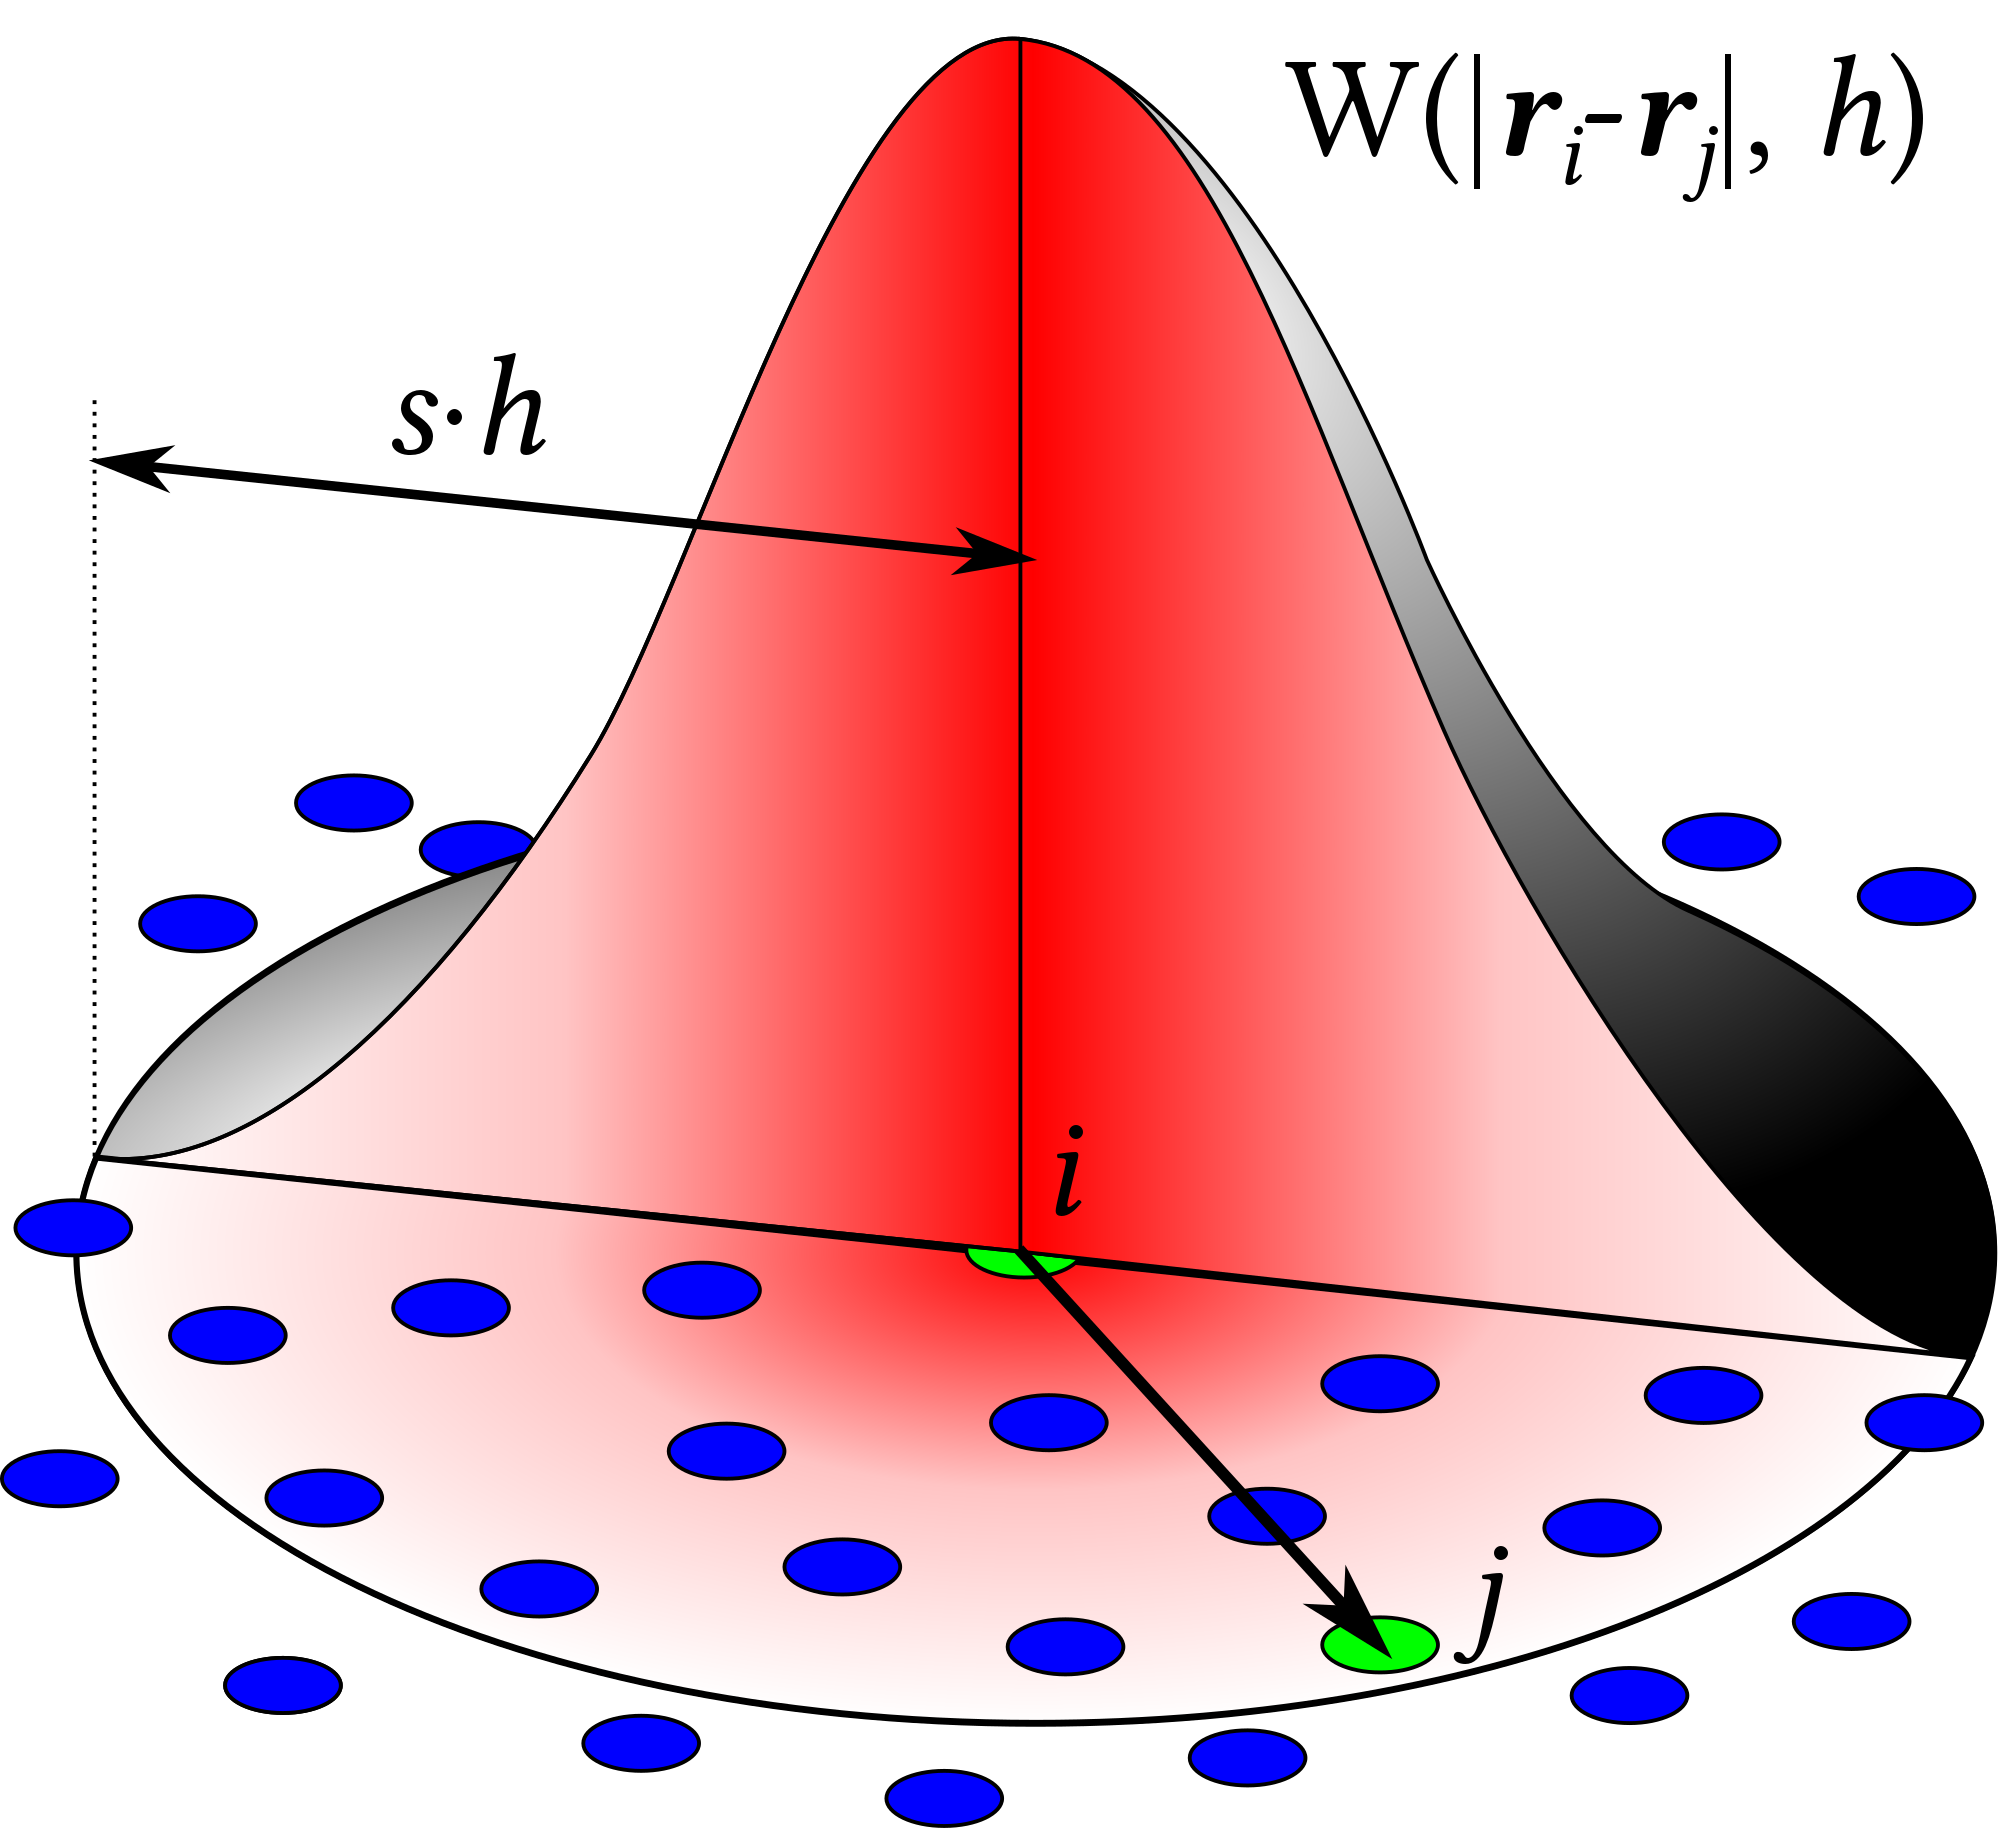
\includegraphics[width=0.5\textwidth]{smoothing_kernel.png}
    \caption{Kernel function \cite{image:smoothing_kernel}}
    \label{fig:smoothing_kernel}
\end{figure}

\subsubsection{Smoothing length}
- can be variable -> great strength of SPH
\begin{equation}
    \frac{\mathrm{d}h}{\mathrm{d}t} = \frac{h}{d}\frac{\partial v^{\alpha}}{\partial x^{\alpha}}
\end{equation}

\subsubsection{Artificial viscosity}
- what it is
- why it is needed
\begin{equation}
    {\frac {\mathrm {d} {\vec {v}}_{a}}{\mathrm {d} t}}=-\sum \limits _{b}m_{b}\left({\frac {P_{b}}{\rho _{b}^{2}}}+{\frac {P_{a}}{\rho _{a}^{2}}}+\Pi _{ab}\right)\nabla _{a}W_{ab}
\end{equation}

\subsubsection{Time Integration}
- second order embedded Runge Kutta with adaptive timestep and relative error (precision) of 10e-6

- Schaefer 2016 3.4.2

Once the partial differential equations are broken down into first order ordinary differential equations in time these equations still need to be solved. There are several well known techniques available to do so. In the simulations for this study a 3rd order Runge-Kutta solver with an adaptive timestep has been used. Runge-Kutta is an explicit method which uses
\begin{equation}
    aaa
\end{equation}


\subsection{Initial conditions}
\subsubsection{Particle setup}
- Target basalt halfsphere \\
- Impactor aluminium sphere \\
- resolution bound to variable smoothing length \\
- Uniform macro structure but random micro structure to avoid \\
- seagen \cite{github:SEAGen} used to create initial conditions
- material density and h have to fit together

\begin{figure}[H]
    \centering
    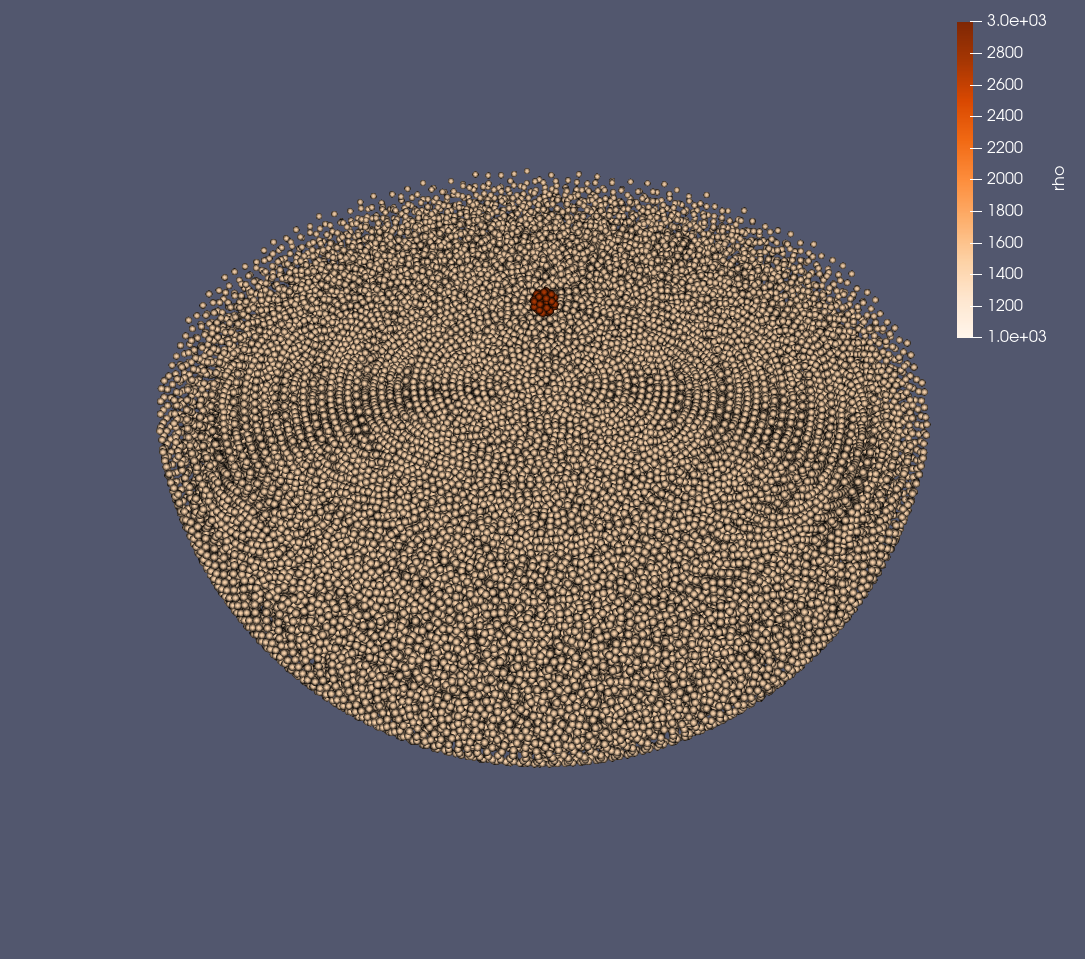
\includegraphics[width=\textwidth]{impact_start.png}
    \caption{start of example simulation}
    \label{fig:impact_start}
\end{figure}

\begin{figure}[H]
    \centering
    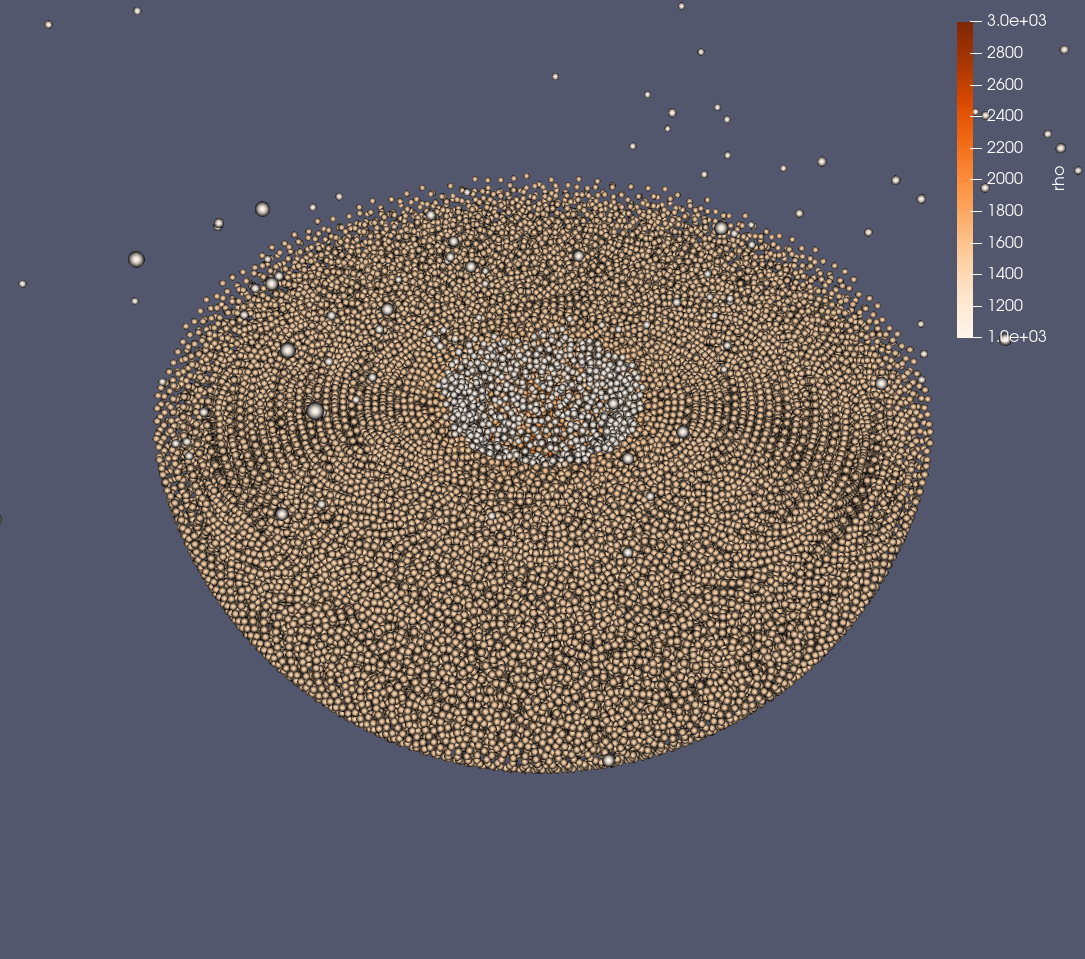
\includegraphics[width=\textwidth]{impact_end.png}
    \caption{end of example simulation}
    \label{fig:impact_end}
\end{figure}

\subsubsection{Material parameters} \label{sect:material_parameters}

\begin{table}
    \centering
    \begin{tabular}{ |l|l|l|l| }
        \hline
        \multicolumn{2}{|c|}{}                & Target                  & Projectile                                                          \\
        \hline
        \multirow{10}{*}{Tillotson EOS}       & $\rho_0$                & 2.86 $\cdot 10^3 g\cdot cm^{-3}$ & 2.70 $\cdot 10^3 g\cdot cm^{-3}$ \\
                                              & $A_T$                   & 2.67 $\cdot 10^{10}$ Pa          & 7.52 $\cdot 10^{10}$ Pa          \\
                                              & $B_T$                   & 2.67 $\cdot 10^{10}$ Pa          & 6.50 $\cdot 10^{10}$ Pa          \\
                                              & $E_0$                   & 4.87 $\cdot 10^8$ $Jkg^{-1}$     & 5.00 $\cdot 10^6$ $Jkg^{-1}$     \\
                                              & $E_{iv}$                & 4.72 $\cdot 10^6$ $Jkg^{-1}$     & 3.00 $\cdot 10^6$ $Jkg^{-1}$     \\
                                              & $E_{cv}$                & 1.82 $\cdot 10^7$ $Jkg^{-1}$     & 1.39 $\cdot 10^7$ $Jkg^{-1}$     \\
                                              & $a_T$                   & 0.5                              & 0.5                              \\
                                              & $b_T$                   & 1.5                              & 1.63                             \\
                                              & $\alpha_T$              & 5.0                              & 5.0                              \\
                                              & $\beta_T$               & 5.0                              & 5.0                              \\ \hline
        \multirow{7}{*}{Porosity}             & $\alpha_0$              & \textbf{varying}                 & not porous                       \\
                                              & $p_{e}$                 & 1.0 $\cdot 10^6$ Pa              & not porous                       \\
                                              & $p_{s}$                 & 2.13 $\cdot 10^8$ Pa             & not porous                       \\
                                              & $c_e$                   & 100.0 $m\cdot s^{-1}$            & not porous                       \\ \hline
        \multirow{6}{*}{Strength}             & cohesive strength $Y_c$ & \textbf{varying}                 & 1.0 $\cdot 10^9$ Pa              \\
                                              & $\alpha_{intact}$       & 0.982793 rad                     & 0 rad                            \\
                                              & $\alpha_{damaged}$      & 0.540419 rad                     & 0 rad                            \\
                                              & shear modulus $\mu$     & 2.27 $\cdot 10^{10}$ Pa          & 2.69 $\cdot 10^{10}$ Pa          \\
                                              & bulk modulus $K_0$      & 2.67 $\cdot 10^{10}$ Pa          & 5.23 $\cdot 10^{10}$ Pa          \\
                                              & shear strength $Y_M$    & 3.5 $\cdot 10^9$ Pa              & 2.76 $\cdot 10^8$ Pa             \\ \hline
        \multirow{3}{*}{Fracture}             & Weibull m               & 16                               & no damage                        \\
                                              & Weibull k               & 1.0 $\cdot 10^{61}$              & no damage                        \\
                                              & Initial damage $d_0$    & 0                                & no damage                        \\  \hline
        \multirow{2}{*}{Artificial viscosity} & $\alpha$                & 1.0                              & 1.0                              \\
                                              & $\beta$                 & 2.0                              & 2.0                              \\ \hline
        \hline
    \end{tabular}
    \caption{Material parameters for basalt target and aluminium Impactor}
    \label{tab:material_parameters}
\end{table}

- variable smoothing length min 0.1 bis max 10.0
- rholimit 0.95
\newpage
\section{Results}
The simulations were run with porosities of 0\%, 17\%, 33\% and 50\% and cohesive strengths of 1kPa, 10kPa, 100kPa and 1MPa under impact angles of 0 and 45 degrees. This yields 32 simulations in total.

\subsection{Cratering}
- qualitative analysis

- head on
\begin{figure}[H]
   \centering
   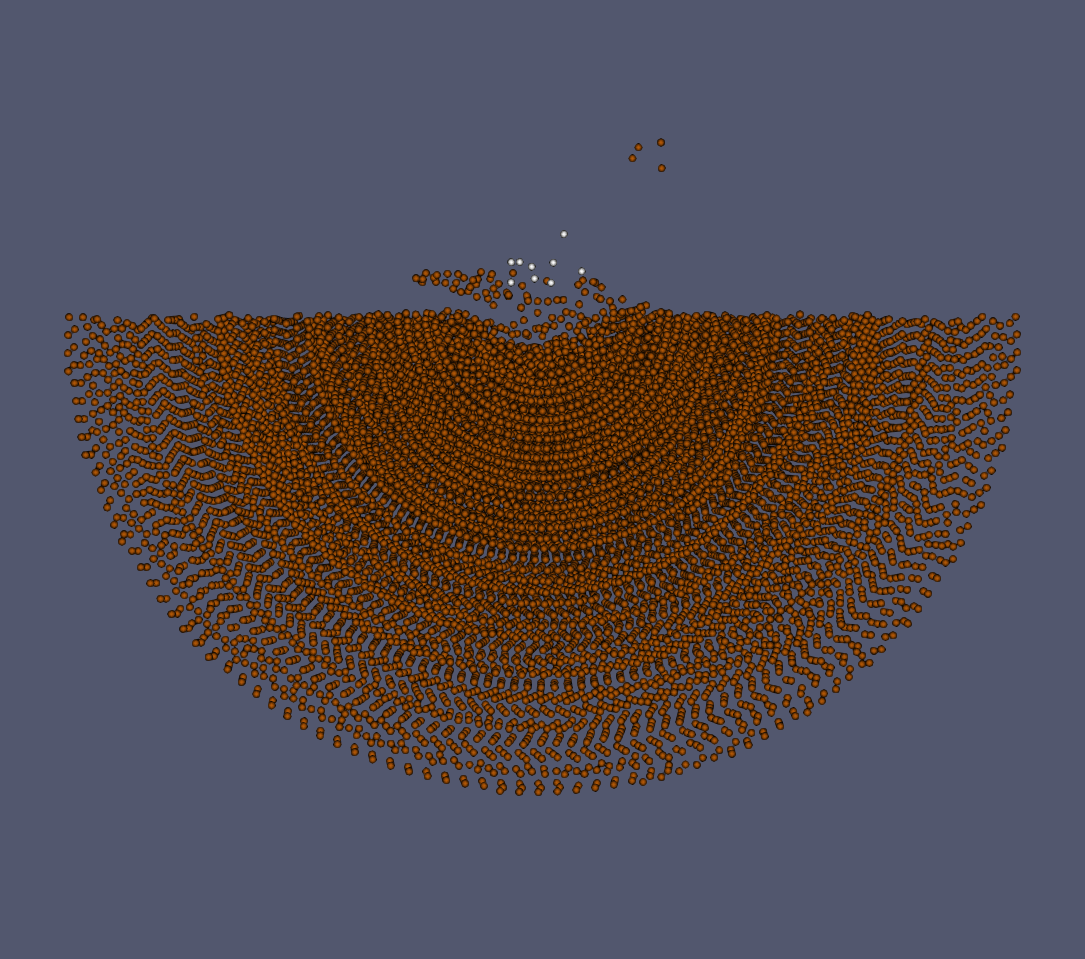
\includegraphics[width=\textwidth]{crater_por0_stre6.png}
   \caption{No porosity (0\%), high strength (Y=1MPa)}
   \label{fig:crater1}
\end{figure}


\begin{figure}[H]
   \centering
   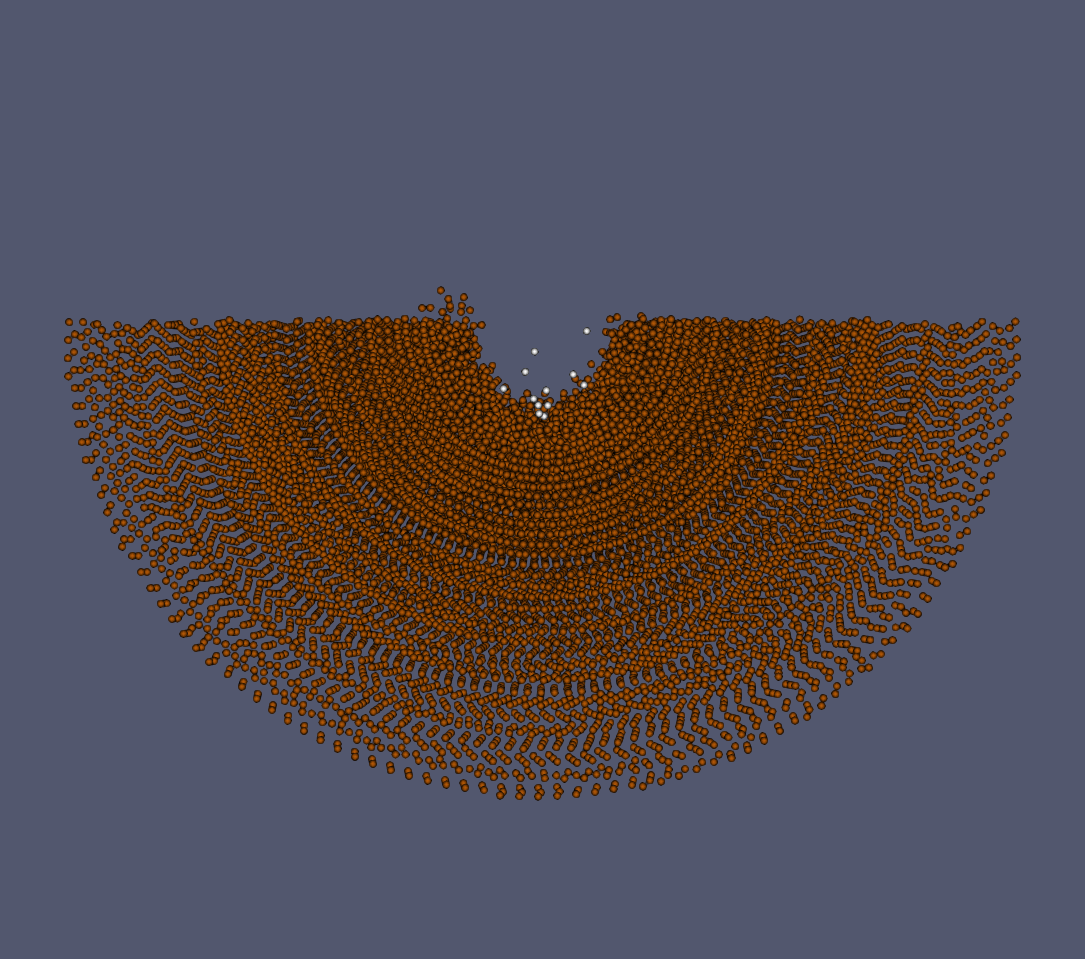
\includegraphics[width=\textwidth]{crater_por50_stre6.png}
   \caption{High porosity (50\%), high strength (Y=1MPa)}
   \label{fig:crater2}
\end{figure}

\begin{figure}[H]
   \centering
   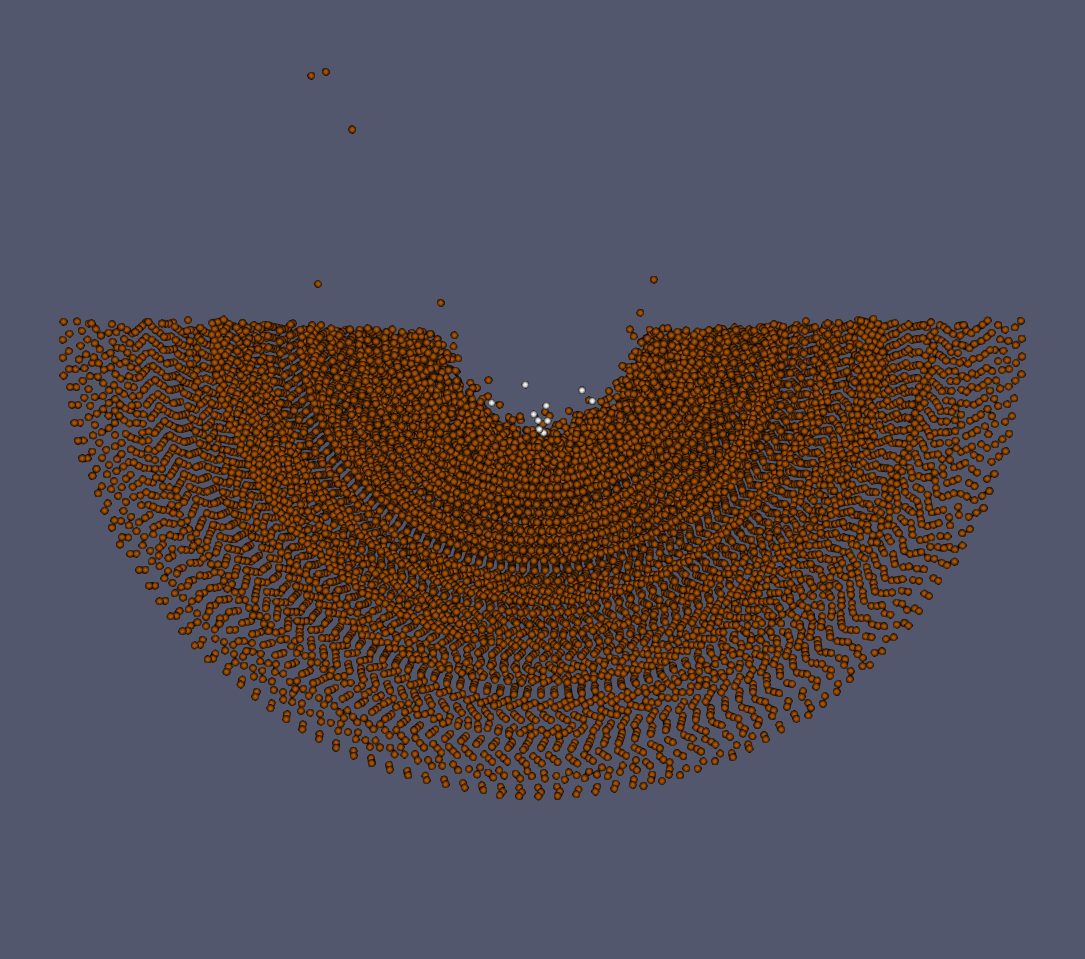
\includegraphics[width=\textwidth]{crater_por50_stre3.png}
   \caption{High porosity (50\%), low strength (Y=1kPa)}
   \label{fig:crater3}
\end{figure}

- 45 degrees
\begin{figure}[H]
   \centering
   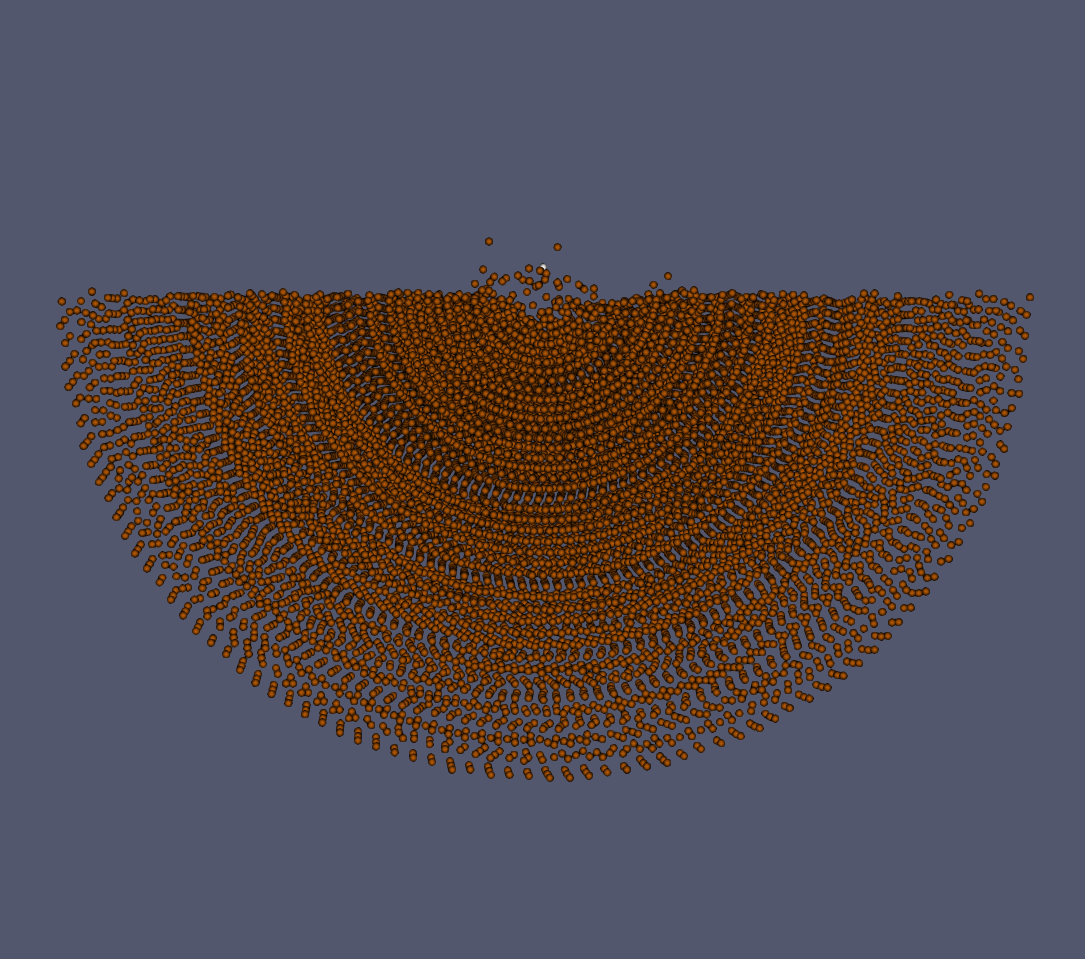
\includegraphics[width=\textwidth]{crater_por0_stre6_ang45.png}
   \caption{No porosity (0\%), high strength (Y=1MPa), 45 degree angle}
   \label{fig:crater4}
\end{figure}


\begin{figure}[H]
   \centering
   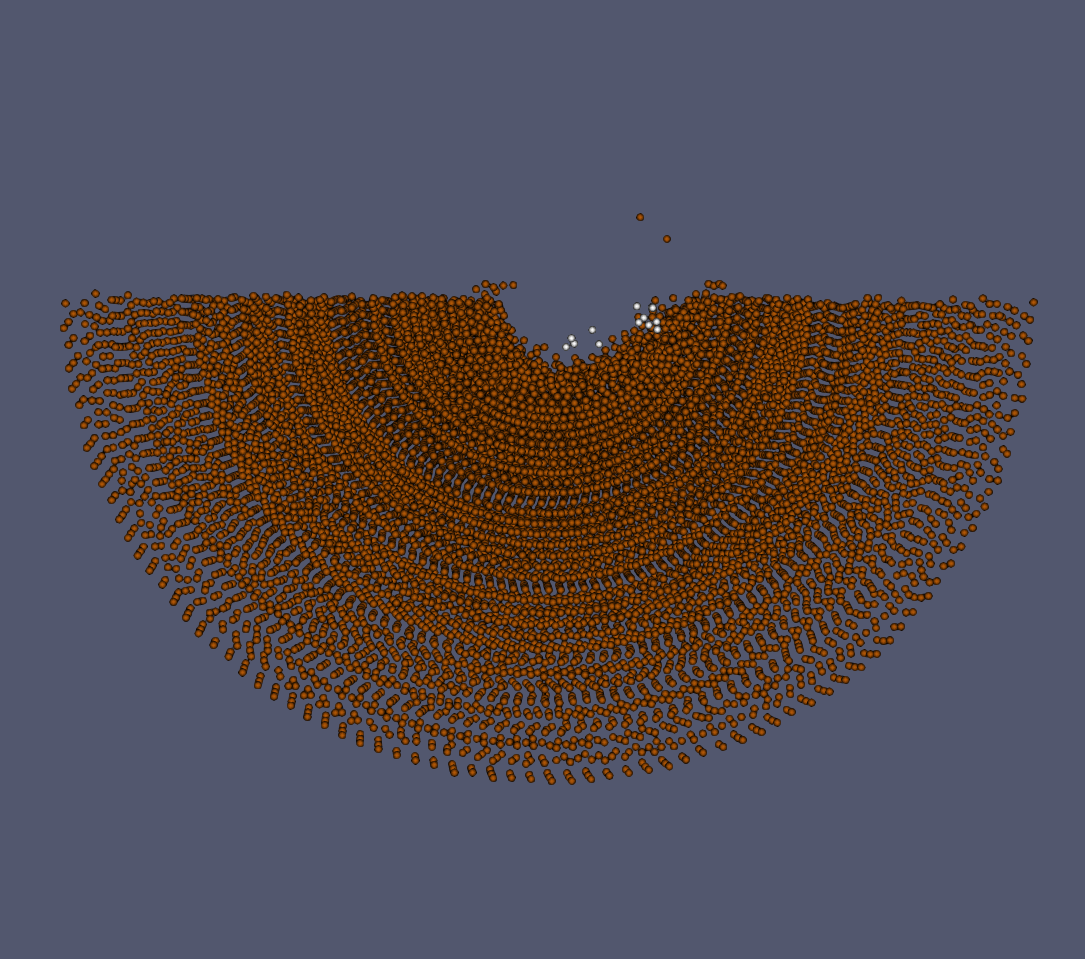
\includegraphics[width=\textwidth]{crater_por50_stre6_ang45.png}
   \caption{High porosity (50\%), high strength (Y=1MPa), 45 degree angle}
   \label{fig:crater5}
\end{figure}

\begin{figure}[H]
   \centering
   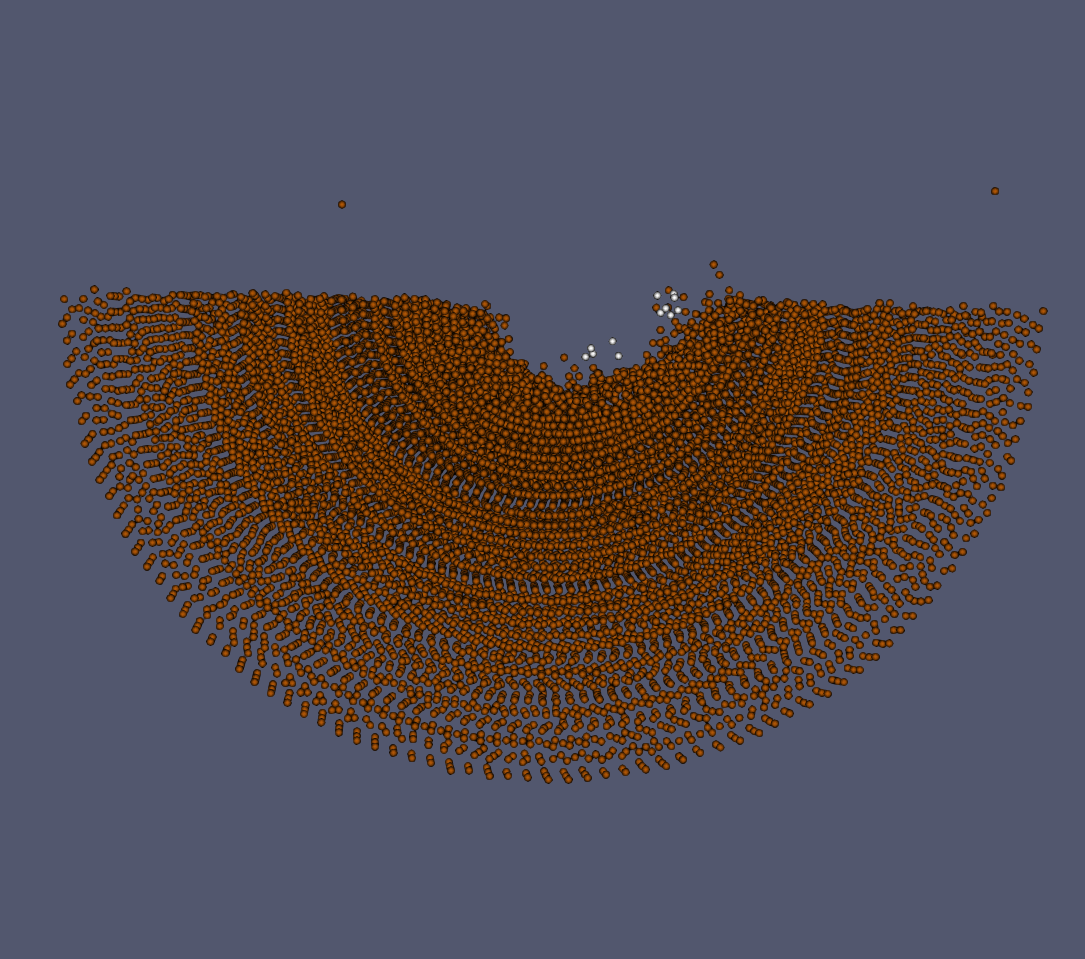
\includegraphics[width=\textwidth]{crater_por50_stre3_ang45.png}
   \caption{High porosity (50\%), low strength (Y=1kPa), 45 degree angle}
   \label{fig:crater6}
\end{figure}

\subsection{Damage}

\begin{figure}[H]
   \centering
   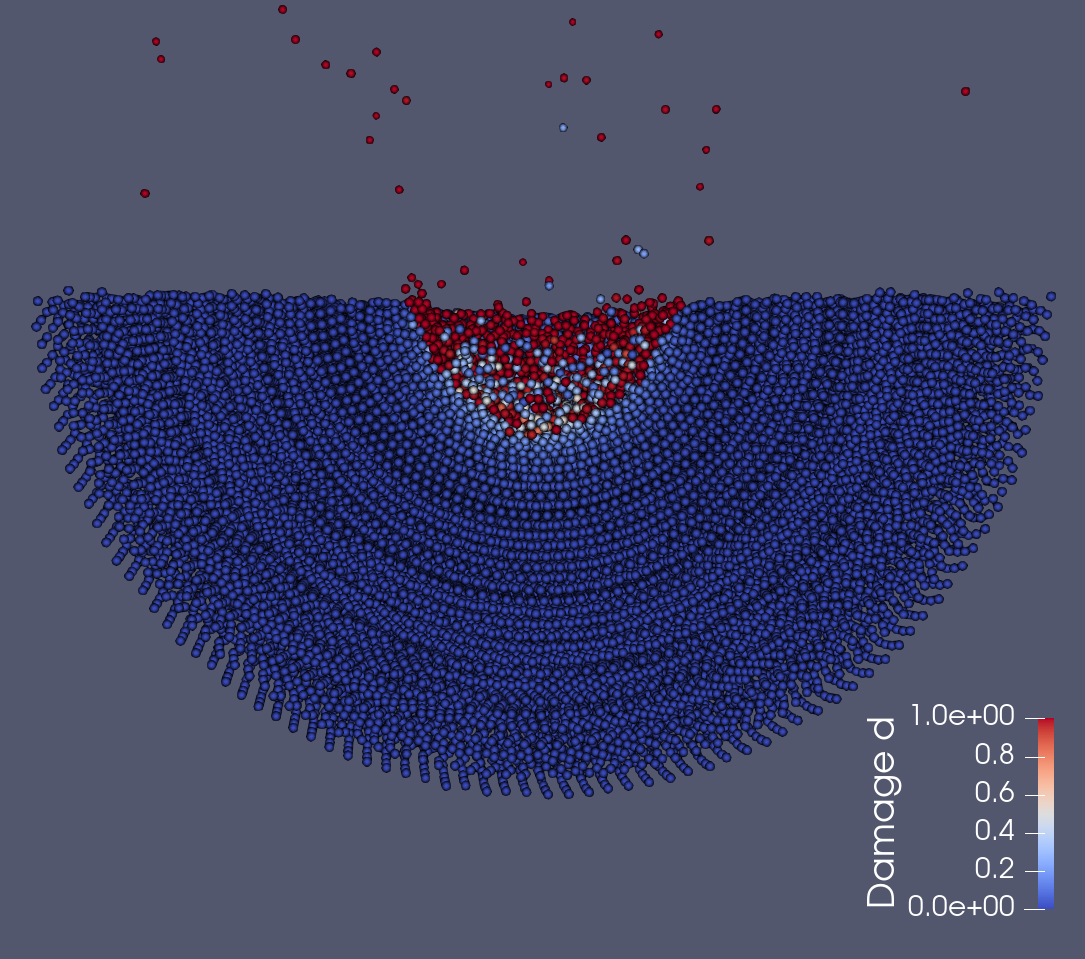
\includegraphics[width=\textwidth]{damage_por50_stre3.png}
   \caption{Damage high porosity (50\%), low strength (Y=1kPa)angle}
   \label{fig:crater6}
\end{figure}

\begin{figure}[H]
   \centering
   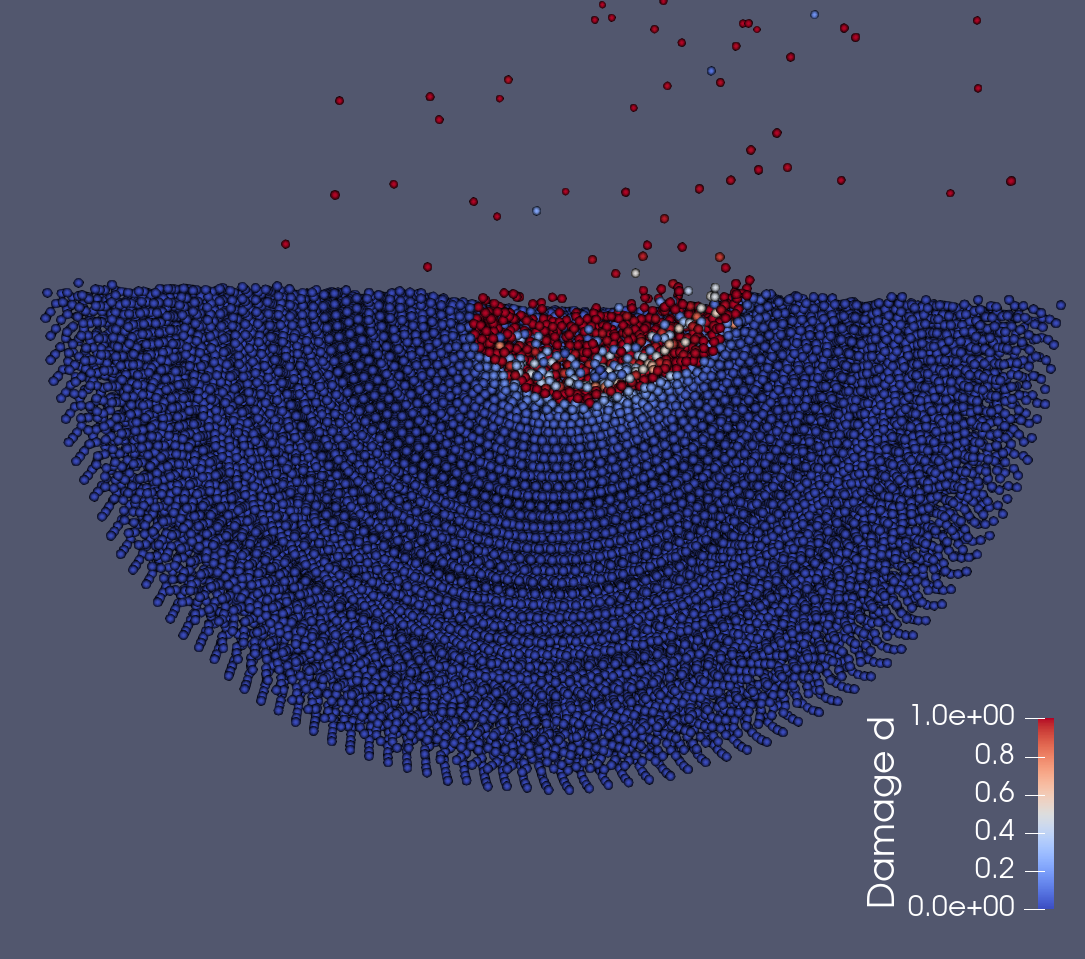
\includegraphics[width=\textwidth]{damage_por50_stre3_ang45.png}
   \caption{Damage high porosity (50\%), low strength (Y=1kPa), 45 degree angle}
   \label{fig:crater6}
\end{figure}

\subsection{Distention}

\begin{figure}[H]
   \centering
   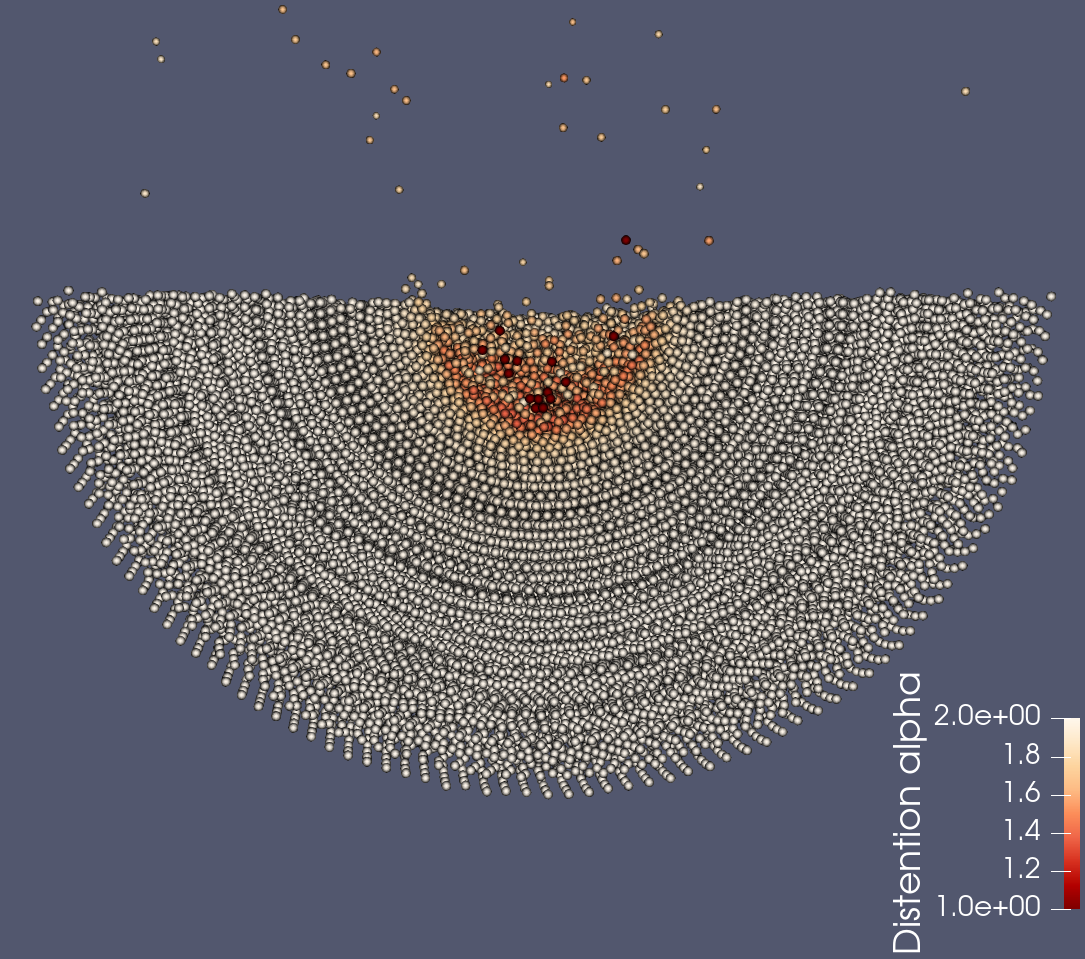
\includegraphics[width=\textwidth]{distention_por50_stre3.png}
   \caption{Distention high porosity (50\%), low strength (Y=1kPa)angle}
   \label{fig:crater6}
\end{figure}

\begin{figure}[H]
   \centering
   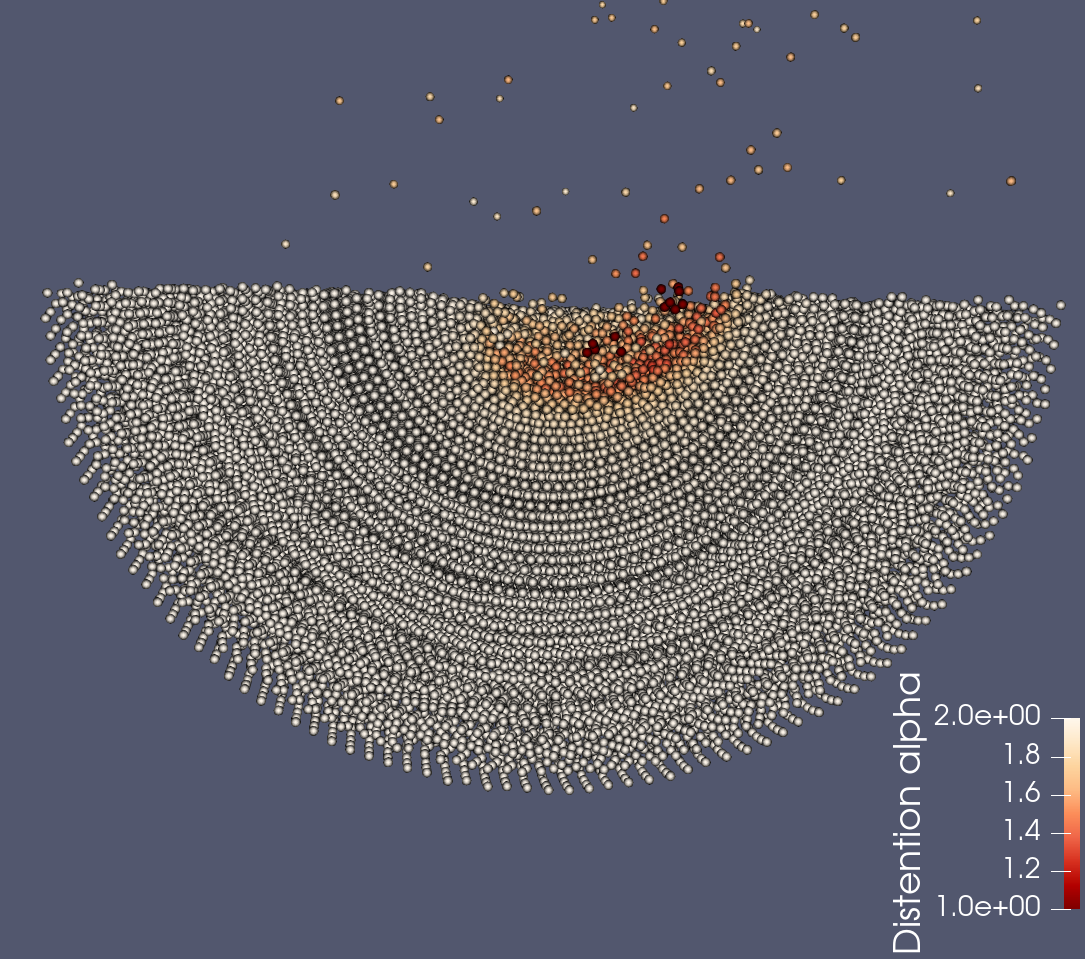
\includegraphics[width=\textwidth]{distention_por50_stre3_ang45.png}
   \caption{Distention high porosity (50\%), low strength (Y=1kPa), 45 degree angle}
   \label{fig:crater6}
\end{figure}

\subsection{Beta factor}
- explanation of beta factor

\begin{figure}[H]
   \centering
   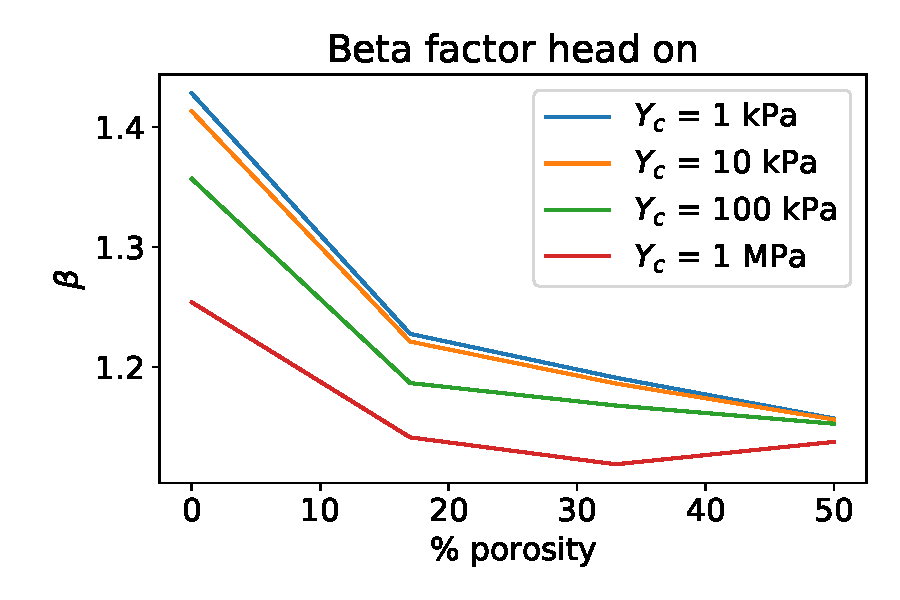
\includegraphics[width=\textwidth]{beta_results_ang0.pdf}
   \caption{beta factor}
   \label{fig:beta_factor_0}
\end{figure}

\begin{figure}[H]
   \centering
   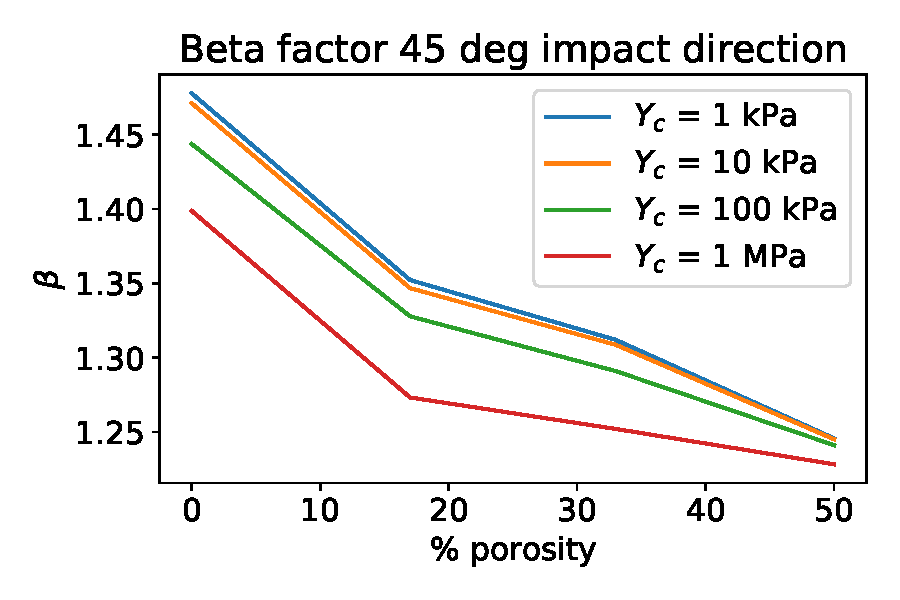
\includegraphics[width=\textwidth]{beta_results_ang45_impact.pdf}
   \caption{beta factor in impact direction}
   \label{fig:beta_factor_45_impact}
\end{figure}

\begin{figure}[H]
   \centering
   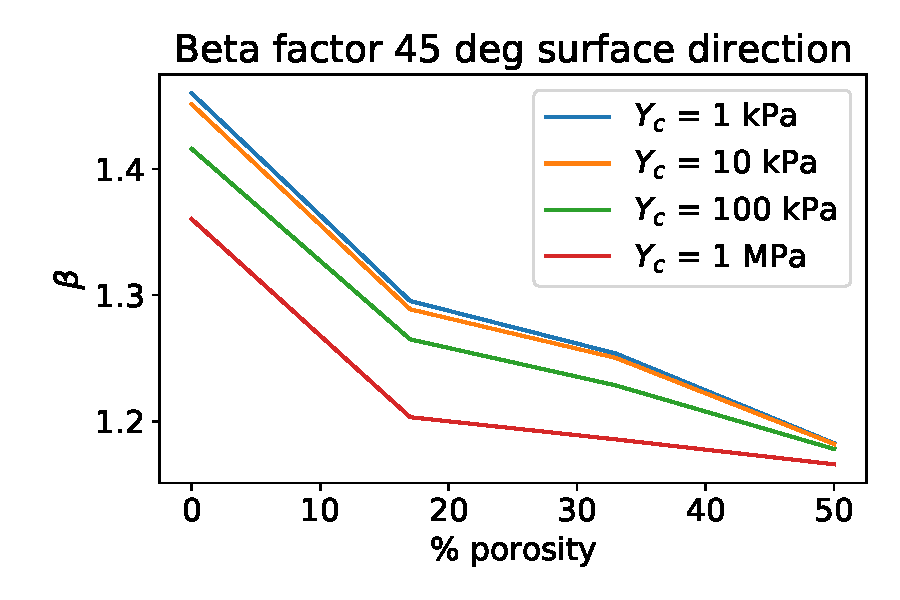
\includegraphics[width=\textwidth]{beta_results_ang45_surface.pdf}
   \caption{beta factor perpendicular to surface}
   \label{fig:beta_factor_45_surface}
\end{figure}

- only particles with positive velocity along impact direction above escape velocity
\begin{equation}
   v_{esc} = \sqrt{\left(\dfrac{2GM}{r_i}\right)}
\end{equation}
where $M = \frac{4}{3}\pi R^3 \rho_{asteroid}$ is the estimated mass of asteroid with R = 75m and $\rho{asteroid}$ = 2.8$\frac{g}{cm^3}$ and $r_i$ distance of sph particle from center of estimated asteroid sphere
- few particles (with highest velocities so the ones that are far away) account for most of the momentum

\begin{figure}[H]
   \centering
   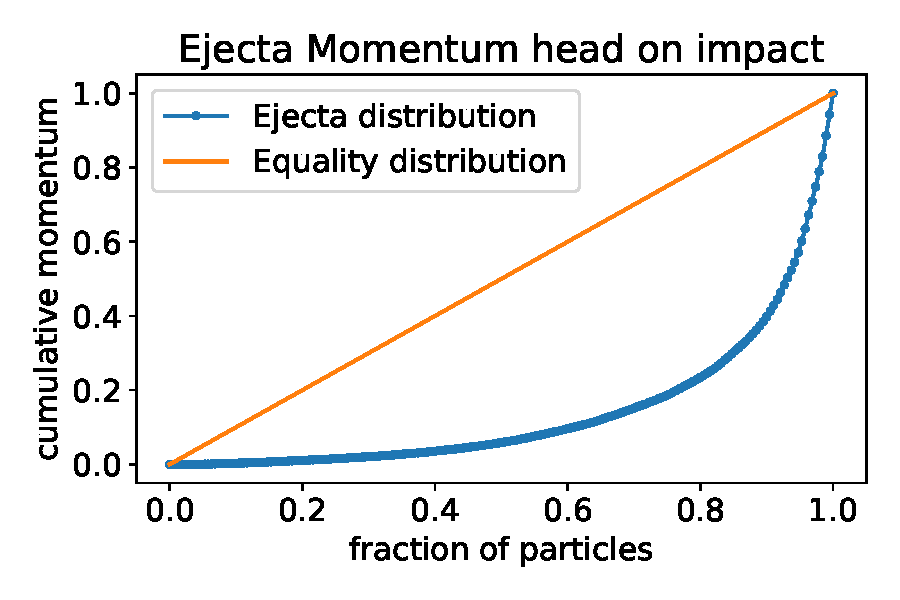
\includegraphics[width=\textwidth]{beta_lorenz_ang0.pdf}
   \caption{Lorenz curve for momentum distribution head on}
   \label{fig:beta_factor_lorenz_0}
\end{figure}

\begin{figure}[H]
   \centering
   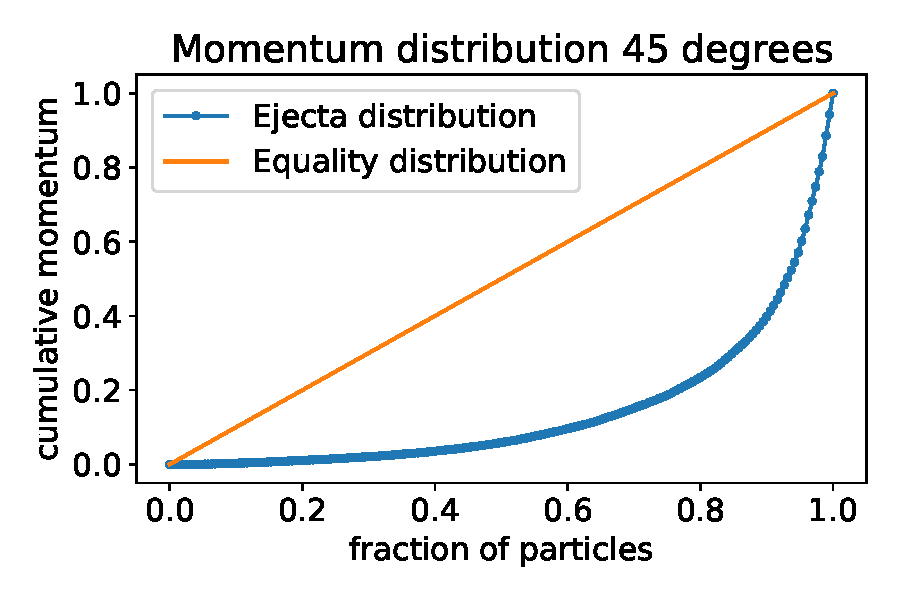
\includegraphics[width=\textwidth]{beta_lorenz_ang45.pdf}
   \caption{Lorenz curve for momentum distribution 45 degree}
   \label{fig:beta_factor_lorenz_45}
\end{figure}
\newpage
\section{Discussion}
- beta factor on the lower end
- upper limit beta < 2 because of momentum conservation??

% References
\newpage
\printbibliography

\end{document}